\begin{frame}
    \frametitle{Áp dụng WWO vào bài toán SO-MKNAP}
    \begin{block}{Phát biểu bài toán:}
        Cho một danh sách gồm $n$ vật thể và $m$ túi. Mỗi vật thể $i$ ($1 \le i \le n$) có trọng lượng trong túi $j$ ($1 \le i \le m$) là $w_{ij}$ và có giá trị là $v_i$. Mỗi túi $j$ có trọng lượng là $c_j$. Chọn ra một tập con các vật thể sao cho chúng vừa tất cả các túi và tổng giá trị là lớn nhất.
    \end{block}
    Ở bài toán này tác giả của bài báo đã sử dụng các phương pháp sau: Lời giải $\mathbf{x}$ sẽ là một vector gồm $n$ giá trị $[0, 1]$. Toán tử lan truyền sẽ sử dụng phép lật bit. Phương trình \hyperlink{eq:e3}{3}, \hyperlink{eq:e4}{4},  \hyperlink{eq:e5}{5} và \hyperlink{eq:e6}{6} được sử dụng để cập nhật bước sóng qua từng thế hệ. Lời giải lan truyền nếu tốt hơn lời gian cũ thì lời giải cũ sẽ bị thay thế. Cuối cùng, số lượng lời giải trong quần thể sẽ bị giảm đi tuyến tính qua từng thế hệ, loại bỏ nhưng lời giải tệ nhất ra khỏi quần thể. Ngoài ra, ở bước vỡ sóng, nhóm tác giả cũng đã thử nghiệm bằng cách linh động chọn ra một trong ba toán tử: loại bỏ lời giải tệ nhất thứ $k$; thêm một vật phẩm có hệ số giá trị cao; và hoán đổi hai vật phẩm được chọn và chưa được chọn sao cho tổng giá trị là cao hơn.
\end{frame}

% \begin{frame}[fragile] 
%     \frametitle{Mã giả thuật toán Tối ưu sóng nước (WWO)}
%     \scriptsize
%     \begin{figure}
%         \begin{algorithm}[H]
%             \caption{Tối ưu sóng nước (Water Wave Optimization)}
%             \label{alg:wwo}
%             \begin{algorithmic}[1]
%                 \State Khởi tạo ngẫu nhiên một quần thể gồm $NP$ lời giải cho bài toán;
%                 \State Đặt $x^*$ là lời giải tốt nhất trong quần thể;
%                 \While{điều kiện dừng chưa thỏa mãn}
%                     \State Tính toán bước sóng $\lambda$ cho mỗi lời giải;
%                     \For{mỗi lời giải $x$ trong quần thể}
%                         \State $k \gets \text{rand}(1, \lambda_x)$;
%                         \State Tạo lời giải mới $x'$ bằng cách đảo ngẫu nhiên $k$ thành phần của $x$;
%                         \If{$f(x') > f(x)$}
%                             \State Thay thế $x$ bằng $x'$ trong quần thể;
%                             \If{$f(x) > f(x^*)$}
%                                 \State Thực hiện tìm kiếm cục bộ quanh $x$;
%                                 \State Cập nhật $x^*$ là lời giải tốt nhất giữa $x$ và các lân cận;
%                             \EndIf
%                         \EndIf
%                     \EndFor
%                     \State Cập nhật kích thước quần thể;
%                 \EndWhile
%                 \State \Return $x^*$
%             \end{algorithmic}
%         \end{algorithm}
%     \end{figure}
% \end{frame}

\begin{frame}[fragile] 
    \frametitle{Mã giả thuật toán Tối ưu sóng nước (WWO)}
    \begin{figure}
        % Scale the entire box containing the algorithm
        \scalebox{0.7}{
            \begin{minipage}{\linewidth}
                \begin{algorithm}[H]
                    % The caption should be inside the environment it's describing
                    \caption{Tối ưu sóng nước (Water Wave Optimization)}
                    \label{alg:wwo}
                    \begin{algorithmic}[1]
                        \State Khởi tạo ngẫu nhiên một quần thể gồm $NP$ lời giải cho bài toán;
                        \State Đặt $\mathbf{x}^*$ là lời giải tốt nhất trong quần thể;
                        \While{điều kiện dừng chưa thỏa mãn}
                            \State Tính toán bước sóng $\lambda$ cho mỗi lời giải;
                            \For{mỗi lời giải $\mathbf{x}$ trong quần thể}
                                \State $k \gets \text{rand}(1, \lambda_\mathbf{x})$;
                                \State Tạo lời giải mới $\mathbf{x}'$ bằng cách đảo ngẫu nhiên $k$ thành phần của $\mathbf{x}$;
                                \If{$f(\mathbf{x}') > f(\mathbf{x})$}
                                    \State Thay thế $\mathbf{x}$ bằng $\mathbf{x}'$ trong quần thể;
                                    \If{$f(\mathbf{x}) > f(\mathbf{x}^*)$}
                                        \State Thực hiện tìm kiếm cục bộ quanh $\mathbf{x}$;
                                        \State Cập nhật $\mathbf{x}^*$ là lời giải tốt nhất giữa $\mathbf{x}$ và các lân cận;
                                    \EndIf
                                \EndIf
                            \EndFor
                            \State Cập nhật kích thước quần thể;
                        \EndWhile
                        \State \Return $\mathbf{x}^*$
                    \end{algorithmic}
                \end{algorithm}
            \end{minipage}
        }
    \end{figure}
\end{frame}

\begin{frame}
    \frametitle{Kết quả thực nghiệm của tác giả}
    \begin{figure}
        \centering
        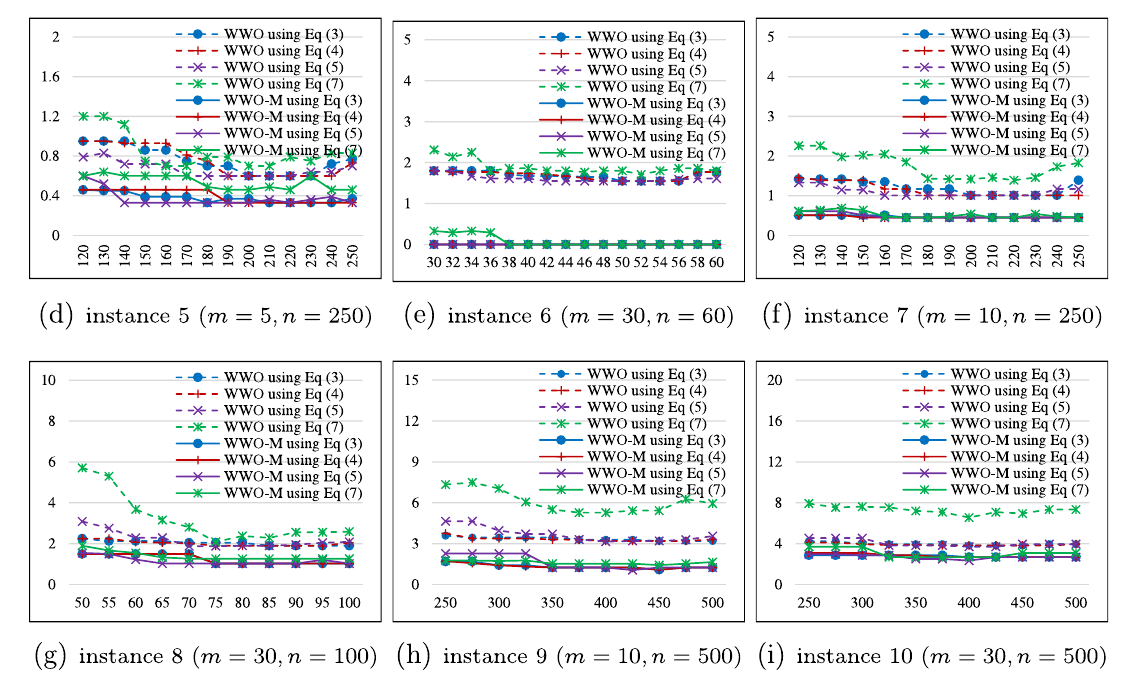
\includegraphics[width=0.7\linewidth]{images/author-mkp-rpd.png}
        \caption{Sai lệch giữa kết quả tốt nhất theo từng thế hẹ và optimal của instance (test case)\cite{zheng2019water}}
        \label{fig:author-mkp-rpd}
    \end{figure}
\end{frame}

\begin{frame}
    \frametitle{Kết quả thực nghiệm của tác giả}
    \begin{figure}
        \centering
        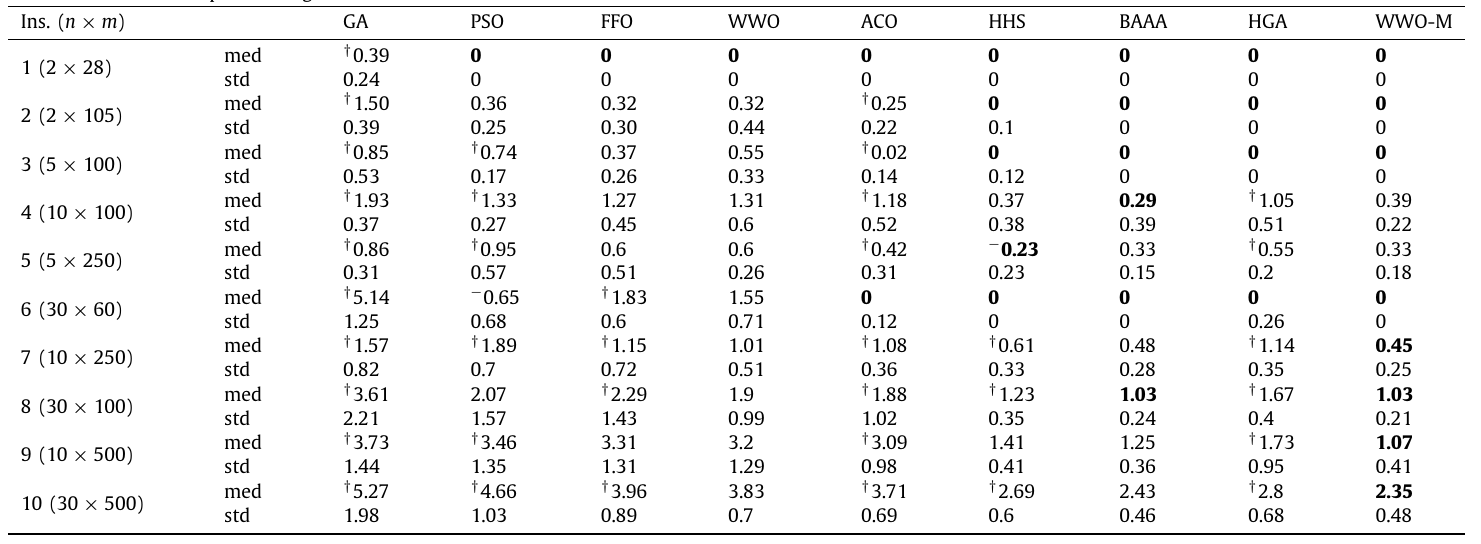
\includegraphics[width=1\linewidth]{images/authors-mkp.png}
        \caption{So sánh giữa các thuật toán heuristic \cite{zheng2019water}}
        \label{fig:authors-mkp}
    \end{figure}
\end{frame}

